% !TeX root = ../main.tex

\chapter{System Design and Implementation}\label{chapter:Persistent Threads}

This thesis initially aimed to bring GPU coroutine support to the open source autonomous driving platform Apollo, by implementing the LuisaCompute-Coroutines framework discussed in Chapter~\ref{chapter:Related Work}.
The goal was to extend Apollo’s existing CPU coroutine infrastructure to GPUs, providing fine-grained, predictable scheduling for real-time tasks.
However, due to integration challenges and the constraints of the project timeline, directly implementing LuisaCompute-Coroutines proved infeasible.
Consequently, the scope shifted toward a manual implementation: a persistent thread scheduler for GPUs that lays the groundwork for coroutine support while still enabling fine-grained control over GPU execution.
This section presents the design and implementation of that scheduler and the foundation it provides for future coroutine integration.

\section{Platform Integration: GPU Scheduling in Apollo}

This thesis initially explored integrating LuisaCompute-Coroutines into Apollo, aiming to provide GPU coroutines to complement the existing CyberRT CPU coroutines.
Similar to the CPU coroutines, these GPU coroutines were intended to deliver predictable execution latencies, with the added latency improvements that GPU persistent threads offer. 
However, due to several integration barriers, including foreign build systems, sparse documentation, time constraints, and a limited familiarity with both projects, GPUs, and compiler theory, it became clear that integrating this system into Apollo would not be feasible within the scope of this thesis.

With the LuisaCompute's coroutines approach impractical, the focus shifted to implementing manual GPU scheduling functionality. 
Finding no suitable open source implementation for coroutines, this thesis instead turned to persistent threads.
Most existing persistent thread implementations are highly application specific and not readily available, which meant that adapting any implementation required substantial work.
The only suitable implementation found was LightKer, a research project designed to measure the speedup of using persistent threads compared to sequential kernel launches. 
To implement LightKer into a real time system, the project required a complete restructuring of the codebase. 
Although full integration into Apollo and support for coroutines remains unfinished, this work extends the real time capabilities of LightKer and provides a foundation for future GPU coroutine integration.

The LightKer implementation was primarily designed to measure the performance difference between sequential kernel executions and a persistent kernel implementation.
It constructed simple, trivial kernels and compared the overhead of explicit host launched kernels versus implicit execution within the persistent kernel.
However, the framework does not support runtime features necessary for a fully functional system.
Nonetheless, it provides host device synchronization through a mailbox system and establishes a fundamental foundation for launching persistent kernels, which proved useful in enabling real time support for the system.

\section{System Design and Architectural Overview}

At a high level, there are four key components integrated into the system to enable real time support: the task queue, memory buffers, stream design, and GPU block synchronization.
The task queue is managed, controlled, and allocated by the host, providing the arguments and tasks for the GPU to execute. 
In particular, this implementation of the task queue gives the programmer fine grained opportunities to manually design and schedule workloads. 
The memory buffers serve as an epoch based staging area for input arguments and output results, as well as persistent memory for the further extension of coroutines.
Stream design and GPU block synchronization ensure that the hardware is utilized efficiently, minimizing idle time and improving performance. 

The individual contributions describe above are combined in the system architecture presented below.
The architectural elements discussed form the core of this thesis, with additional tools and synchronization mechanisms, such as the mailbox system, adoped from the LightKernel project.

\begin{figure}[H]
  \centering
  \resizebox{1.0\linewidth}{!}{
	  %\documentclass[tikz, border=5mm]{standalone}
%\usepackage{tikz}
%\usetikzlibrary{shapes, arrows.meta, positioning, decorations.pathreplacing}

%\begin{document}

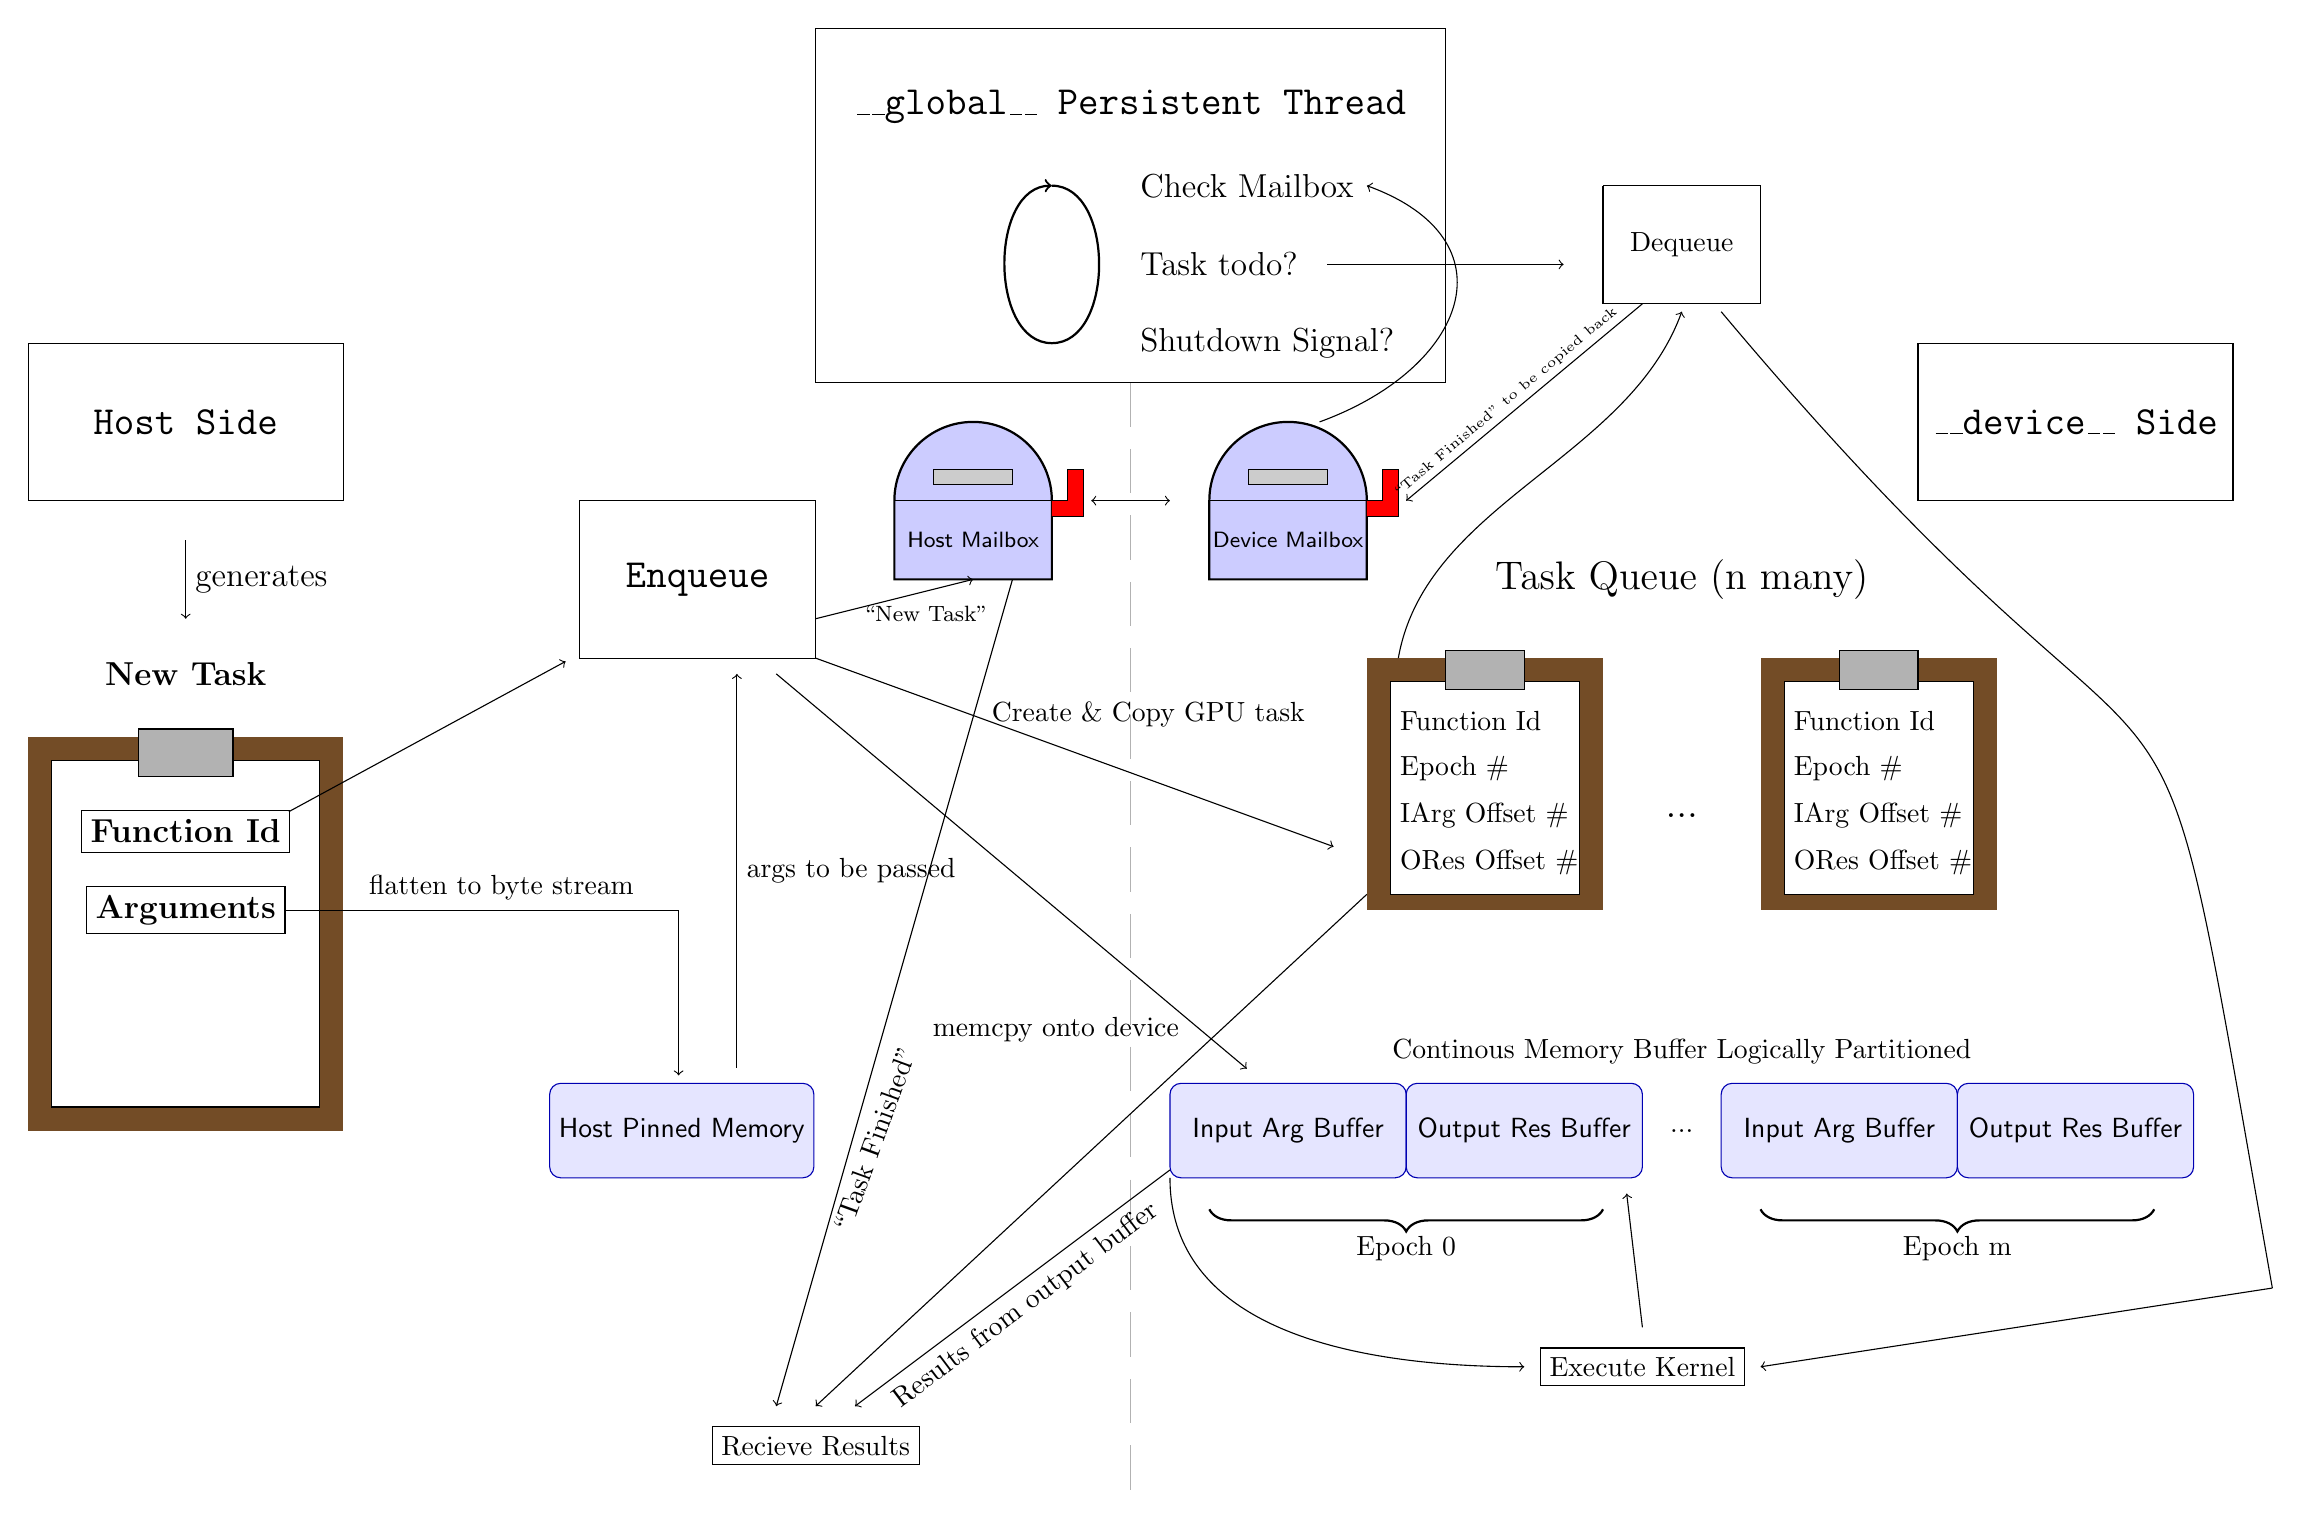
\begin{tikzpicture} [memoryblock/.style={
		draw=blue!70!black, 
		fill=blue!10, 
		rounded corners=4pt, 
		minimum width=3cm, 
		minimum height=1.2cm,
		font=\sffamily
	},
	pinicon/.style={
		symbol/.style={draw, fill=gray!40, symbol color=gray!80, symbol type=pin}
	}
	]

	%\draw[help lines] grid(32,32);


%GLOBAL BOX
	\draw[black] (12,32) -- ++(0:8) -- ++(-90:4.5) -- ++(-180:8) -- ++(-270:4.5);
	\node[minimum size=5] at (16,31) {\Large \texttt{\_\_global\_\_ Persistent Thread}};
	\node[minimum size=8, anchor=west] at (16, 29) {\large Task todo?};
	\node[anchor=west, minimum size=8] at (16, 28) {\large Shutdown Signal?};

	\node[anchor=west, minimum size=8] at (16, 30) {\large Check Mailbox};

	\draw[thick, ->]
	(15, 30)
	.. controls (15.8, 30) and (15.8, 28) .. (15, 28) 
	.. controls (14.2, 28) and (14.2, 30) .. (15, 30); 


	\draw[black, opacity=0.3,  dash pattern=on 16pt off 8pt] (16,27.5) --++(-90:14.2);

%Host Box
	\draw[black] (2, 28) --++(0:4) --++(-90:2) --++(-180:4) --++(-270:2);
	\node[ minimum size=5] at (4,27) {\Large \texttt{Host Side}};
	\draw[black ] (26, 28) --++(0:4) --++(-90:2) --++(-180:4) --++(-270:2);
	\node[ minimum size=5] at (28,27) {\Large \texttt{\_\_device\_\_ Side}};

%HOSTSIDE ARROW
	\draw[->] (4, 25.5) --++ (-90:1) node[pos=0.5, right] {\large generates};
%CLIPBOARD
	\node[font=\bfseries\large] at (4,23.8) {New Task};
	\fill[brown!60!black] (2,23) rectangle (6,18);
	\fill[white] (2.3,22.7) rectangle (5.7,18.3);
	\draw[black] (2.3,22.7) rectangle (5.7,18.3);
	\fill[gray!60] (3.4,23.1) rectangle (4.6,22.5);
	\draw[black] (3.4,23.1) rectangle (4.6,22.5);

	\node[draw, font=\bfseries\large] at (4,21.8) {Function Id};
	\node[draw, font=\bfseries\large] at (4,20.8) {Arguments};


%HOST PINNED MEM
	\node[memoryblock] at (10.3, 18) {Host Pinned Memory};
	\draw[black, ->] (5.26, 20.8) --++ (0: 5) node[pos=0.55, above] {flatten to byte stream} --++(-90: 2.1);


%ENQUEUE
	\draw[black] (9, 26) --++(0:3) --++(-90:2) --++(-180:3) --++(90:2);
	\node[minimum size=5] at (10.5,25) {\Large \texttt{Enqueue}};
	\draw[<-] (11,23.8) --++(-90:5) node[pos = 0.5, right] {args to be passed};
	\draw[->] (11.5,23.8) --++(-40:7.8) node[pos=0.9, left=4pt] {memcpy onto device};
	\draw[->] (5.31, 22.05) --++ (28.5:4);
	\draw[->] (12, 24) --++ (-20:7) node[pos=0.3,right=4pt] {Create \& Copy GPU task};


%MAILBOX HOST
	\draw[<->] (15.5, 26) -- (16.5, 26);
	\draw[thick, fill=blue!20] (13,25) -- (13,26) arc[start angle=180, end angle=0, radius=1cm] -- (15,25) -- cycle;
	\draw[fill=black!20] (13.5,26.2) rectangle (14.5,26.4);
	\draw[fill=red] (15,26) --++(0:0.2)--++(90:0.4)--++(0:0.2)--++(-90:0.6) --++(-180:0.4);
	\node at (14,25.5) {\footnotesize\textsf{Host Mailbox}};
	\draw (13,26) --(15,26);

%MAILBOX DEVICE
	\draw[thick, fill=blue!20] (17,25) -- (17,26) arc[start angle=180, end angle=0, radius=1cm] -- (19,25) -- cycle;
	\draw[fill=black!20] (17.5,26.2) rectangle (18.5,26.4);
	\draw[fill=red] (19,26) --++(0:0.2)--++(90:0.4)--++(0:0.2)--++(-90:0.6) --++(-180:0.4);
	\node at (18,25.5) {\footnotesize\textsf{Device Mailbox}};
	\draw (17,26) --(19,26);

%ARROWS to and FROM DEVICE MAILBOX
	\draw [->] (18.4, 27) to[out=20,in=-20,distance=2.0cm] (19, 30);
	\draw[->] (12, 32-7.5) -- (14,32-7) node[pos=0.7,below=2pt] {\footnotesize{``New Task''}};

%Memory Buffers
	\node at (23, 19) {Continous Memory Buffer Logically Partitioned};
	\node[memoryblock] at (18, 18) {Input Arg Buffer};
	\node[memoryblock] at (21, 18) {Output Res Buffer};

	\node[memoryblock] at (25, 18) {Input Arg Buffer};
	\node[memoryblock] at (28, 18) {Output Res Buffer};

	\node at (23, 18) {...};
	\draw[decorate, decoration={brace,mirror,amplitude=8pt}, thick] (17, 17) -- (22, 17)
	node[midway,below=6pt] {Epoch 0};

	\draw[decorate, decoration={brace,mirror,amplitude=8pt}, thick] (24, 17) -- (29, 17)
	node[midway,below=6pt] {Epoch m};

%TASK QUEUE
	\fill[brown!60!black] (19,24) rectangle (22,20.8);
	\fill[white] (19.3,23.7) rectangle (21.7,21.0);
	\draw[black] (19.3,23.7) rectangle (21.7,21.0);
	\fill[gray!60] (20,24.1) rectangle (21.0,23.6);
	\draw[black] (20,24.1) rectangle (21.0,23.6);

	\node [anchor=west] at (19.3,23.2) {Function Id};
	\node [anchor=west] at (19.3,22.6) {Epoch \#};
	\node [anchor=west] at (19.3,22.0) {IArg Offset \#};
	\node [anchor=west] at (19.3,21.4) {ORes Offset \#};

	\node at (23, 22) {\Large...};

	\fill[brown!60!black] (24,24) rectangle (27,20.8);
	\fill[white] (24.3,23.7) rectangle (26.7,21.0);
	\draw[black] (24.3,23.7) rectangle (26.7,21.0);
	\fill[gray!60] (25,24.1) rectangle (26.0,23.6);
	\draw[black] (25,24.1) rectangle (26.0,23.6);
	\node [anchor=west] at (24.3,23.2) {Function Id};
	\node [anchor=west] at (24.3,22.6) {Epoch \#};
	\node [anchor=west] at (24.3,22.0) {IArg Offset \#};
	\node [anchor=west] at (24.3,21.4) {ORes Offset \#};

	\node at (23,25) {\Large Task Queue (n many)};


%DEQUEUE
	\draw (22, 30) -- (24, 30) --++ (-90:1.5) --++(-180:2) --++ (90:1.5);
	\node at (23, 29.25) {Dequeue};
	\draw[->] (18.5, 29) --++(0:3);
	\draw [->] (19.4, 24) to[out=80,in=-110,distance=2.0cm] (23, 28.4);
	\draw [->] (22.5,28.5) -- (19.5, 26) node[pos=0, left=7pt, rotate=40] {\tiny``Task Finished'' to be copied back};


%EXECUTE Kernel
	\draw (23.5,28.4) to[out=-50, in=100, distance=10.0cm] (30.5,16);
	\draw [->] (30.5,16) -- (24,15);
	\draw [->] (22.5,15.5) -- (22.3,17.2);
	\draw [->] (16.5,17.4) to[out=-90, in=180] (21.0,15.0);
	\node [draw] at (22.5, 15) {Execute Kernel};

%Recieve Result
	\node [draw] at (12, 14) {Recieve Results};
	\draw [->] (19, 21) -- (12, 14.5);
	\draw [->] (16.5, 17.5) -- (12.5, 14.5) node [pos=0.5, below, rotate=37] {Results from output buffer};
	\draw [->] (14.5, 25) -- (11.5, 14.5) node [pos=0.8,right=5pt, rotate=70] {``Task Finished''};

\end{tikzpicture}

%\end{document}


  }
  \caption{Persistent Thread Architecture implemented into LightKer}
  \label{fig:architecture}
\end{figure}


The Figure~\ref{fig:architecture} depicts the individual components in a logical program architectural overview.
The left side of the figure shows the host side code and methods, which handle the enqueuing of tasks and launching of the persistent thread kernel.  
On the right hand side, the device side code is shown, illustrating memory allocation and kernel execution, which processes tasks and writes results back to the memory buffers.  
The mailboxes continuously notify each other of newly enqueuing and dequeuing tasks throughout kernel execution.

The system is initialized by launching the persistent kernel, shown in the uppermost box in Figure\ref{fig:architecture}, which runs for the entire duration of the program. 
The persistent kernel recieves tasks enqueued from the host system, by the transfer of two different objects. 
The first object, is the task itself, represented by a clipboard, which is copied into the task queue. 
The second object is the task memory, serialized by the host and copied into the continuous memory buffer. 
The device is then notified through the mailbox synchronization mechanism and begins executing tasks.
Once a kernel finishes execution, the device notifies the host, which then copies the memory back.

\section{Task Management System}

For persistent threads to execute kernels at runtime, a staging mechanism is required to enqueue tasks and maintain the task context necessary for execution.  
As discussed in Chapter~\ref{chapter:Background}, any task management system that relies on device side scheduling logic is inherently ineffecient due to characteristics of GPU architecture.
Therefore, the task management system in this design adopts a host driven scheduling model, where tasks are prepared and dispatched from the CPU, while persistent threads on the GPU handle execution. 
This approach enables better control over task odering, reduces idle time, and improves overall predictability, essential for real time workloads. 
Furthermore, this system should be compatible with coroutine based execution and priority scheduling in the future. 


\subsection{Task Queue Design}


\begin{figure}[H]
  \centering
  \resizebox{1.0\linewidth}{!}{
	  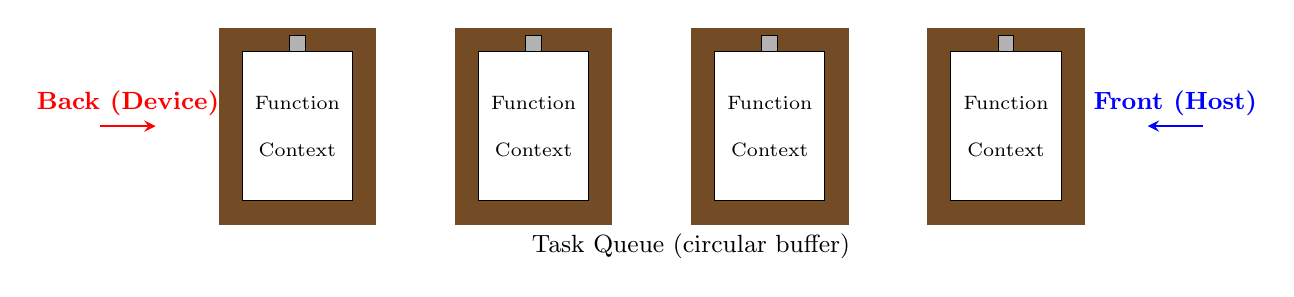
\begin{tikzpicture}[font=\small,>=stealth]

% Number of slots (more spacing)
\foreach \i in {0,1,2,3} {
    \pgfmathsetmacro{\x}{\i * 3} % spacing
    % Clipboard outer
    \fill[brown!60!black] (\x,0) rectangle (\x+2,2.5);
    % Inner white area
    \fill[white] (\x+0.3,0.3) rectangle (\x+1.7,2.2);
    \draw[black] (\x+0.3,0.3) rectangle (\x+1.7,2.2);
    % Gray clip area
    \fill[gray!60] (\x+0.9,2.4) rectangle (\x+1.1,2.2);
    \draw[black] (\x+0.9,2.4) rectangle (\x+1.1,2.2);
    
    % Labels inside
    \node[font=\scriptsize] at (\x+1,1.55) {Function};
    \node at (\x+1,0.95) {\scriptsize Context};
}

% Back pointer (Device) pointing to left side
\draw[thick,->,red] (-1.5,1.25) -- (-0.8,1.25) node[midway,above]{\textbf{Back (Device)}};

% Front pointer (Host) pointing to right side
\draw[thick,->,blue] (12.5,1.25) -- (11.8,1.25) node[midway,above]{\textbf{Front (Host)}};

% Label for queue
\node[below] at (6,0) {Task Queue (circular buffer)};

\end{tikzpicture}

  }
  \caption{GPU Task Queue for Task Management}
  \label{fig:taskqueuearchitecture}
\end{figure}

The architecture implemented into the persistent thread scheduler uses a loop through buffer, as a FIFO queue, in a producer-consumer architecture. 
As shown in Figure~\ref{fig:taskqueuearchitecture}, each GPU task is represented as a clipboard, which contains the function context. 
The context contains both the information needed to execute the device function, as well as metadata for the control of the task within the queue. 
The host acts as a producer, enqueuing tasks into the task queue at the front, while the device consumes tasks from the back.

To improve the complex scheduling efficiency, all task enqueuing and dequeueing logic rests on the host side of the system. 
Enqueuing a task involves copying its context into the task queue and initializing the associated control variables of the task within the function context. 
Before execution, the device simply checks the control variables to ensure that only valid tasks are executed. 
Upon tasks being executed by a \acs{CTA}, the device block will advance the back pointer to the next available task within the queue. 

To ensure that tasks are not overwritten, the host tracks the total number of tasks currently in the system in relation to the total length of the task queue.
Every time a new task is added to the queue, the tracker is incremented, unless the queue is full, which results in a failure response, similar to the native CUDA system. 
For the host to decrement the length tracker, the device must execute the task, notify the host, upon which the host can copy the results back. 
After the results are copied back, a new task can then be enqueued to the same postion in the queue. 



\subsection{Extensibility for Coroutines and Priority Scheduling}

The function contexts stored in the task queue buffer were specifically designed with the future implementations of coroutines and priority scheduling in mind. 
By introducing additional control variables into the function context, the host system can assign tasks different priorities. 
Furthermore, the queue already provides space to store the continuation of the coroutine, allowing a task to yield and record the current instruction for later resumption.

Currently the system executes tasks in a loop using a synchronized busy waiting scheme.
However with slight modifications, it can be extended to support priorities. 
If every task additionally contained a priority or deadline in its function context, the persistent threads polling active tasks could select and execute the most critical tasks first. 
In this case, the host would need to actively track executing tasks to ensure they are not accidently overwritten.

In conjuction with this system, the function context can also store the coroutine continuation.
While precomputed values could be easily stored in the function context, capturing the resumption address is more challenging.  
On the GPU it would be necessary to define specific set points within the program and save a variable in the function context that indicates the next instruction to be executed within the kernel. 


\section{Function Context}

Each task entry defines its execution context through an explicit function identifier and its associated function parameters.
This entry acts exactly like a coroutine continuation, which stores the necessary state to resume execution within the function. 
The function id is used in conjuction with a lookup table to execute the GPU device code. 
The memory location for the parameters is allocated by the host as part of the enqueuing and memory management systems.

\subsection{GPU Function Pointers}

To execute new functions from the persistent threads, the task queue needs to be able to reference the specific function. 
Generally referencing functions on a \acs{CPU} requires only the function pointer to execute the code defined at that memory location. 
When GPU functions are compiled, the device code lives in the GPU address space and is not accessible from the CPU.  
The CPU only has access to functions denoted by the \lstinline[language=cuda]`__global__` keyword, which allows the execution of GPU kernels, not enqueuing of GPU functions.
In order to be able to access and run the functions specified by the CPU, the task queue supports a lookup table to map integers to specific functions.  
The lookup table allows the host to memcpy in function ids to the task queue when enqueuing new tasks.

\subsection{Function Parameters}

When the CPU assigns tasks to the GPU, it passes either allocated GPU memory pointers or explicit parameters. 
These explicit parameters then get propogated to all the individual threads executing the kernel code, resulting in greater api memory overhead. 
When enqueuing new tasks to the task queue, the memory has to be transfered at runtime before the device function calls. 

The GPU task in the queue originally had a pointer to the allocated memory and upon recieving compute resources would schedule the task with the memory to the individual persistent thread.
Unfortunately, this method is dependent on the specific task and parameters and consumes variable memory requiring further pointers to GPU memory.  
In order to consolidate the memory pointers, the task queue was simplified to contain only allocated memory pointers in order to automatically load kernel memory. 

In this method, enqueing the GPU tasks forces the programmer to streamify the data and automatically load the memory into preallocated memory partitions. 
The task queue then only consists of the actual memory partition pointers, both start and end. 
Executing a task then requires the interpretation of the memory and then the loading of it into the device function.
Should the input memory be oversubscribed, the task then has a preallocated buffer to store any updated context for the continuation of the coroutine. 

\section{Memory Management System}


The memory management system supports the task queue, while eliminating unnecessary memory allocation and deallocation overheads. 
By managing memory centrally, the task queue's function contexts can remain simple and flexible. 
This memory system is managed for the lifetime of the persistent kernel, removing the need for costly dynamic memory operations at runtime.  
While maintaining a memory buffer is simple, designing a runtime strategy to partition memory among tasks and reclaim it efficiently presents a more complex challenge. 
To visualize this, Figure~\ref{fig:membuffer} shows the memory buffer logically partitioned into epochs, with each epoch containing input argument and output result buffers for the corresponding tasks.


\subsection{Memory Buffer Design}

\begin{figure}[H]
  \centering
  \resizebox{1.0\linewidth}{!}{
	  \usetikzlibrary{decorations.pathreplacing, positioning}

\begin{tikzpicture}[memoryblock/.style={draw, fill=gray!30, minimum width=3em, minimum height=2em, text centered, font=\small}, node distance=0.3cm]

	% Title

	% Epoch 0
	\node[memoryblock] (in0) at (0,1) {Input Arg Buffer};
	\node[memoryblock, right=0.3cm of in0] (out0) {Output Res Buffer};

	% Ellipsis for intermediate epochs
	\node[right=0.3cm of out0] (dots) {...};

	% Epoch m
	\node[memoryblock, right=0.3cm of dots] (inm) {Input Arg Buffer};
	\node[memoryblock, right=0.3cm of inm] (outm) {Output Res Buffer};

	% Braces for epochs
	\draw[decorate, decoration={brace,mirror,amplitude=8pt}, thick] (in0.south west) -- (out0.south east)
	node[midway,below=6pt, font=\small] {Epoch 0};

	\draw[decorate, decoration={brace,mirror,amplitude=8pt}, thick] (inm.south west) -- (outm.south east)
	node[midway,below=6pt, font=\small] {Epoch m};

\end{tikzpicture}


  }
  \caption{Continuous Memory Buffer Logically Partitioned}
  \label{fig:membuffer}
\end{figure}


The memory management system consists of a single, logically partitioned memory buffer, designed to reduce the complexity of allocation algorithms. 
Each epoch within this buffer contains both an input argument and output result section.
The entire overhead of managing the position of task memory within the buffers is entirely managed by the host and shared with the device through the function context within the task queue. 


As tasks are allocated within the epochs, eventually one of the corresponding memory buffer will overflow. 
When the host detects that allocating memory for a task either results in the input or output buffer overflowing, the host begins allocation in the next epoch.  
After fully allocating the memory for an individual buffer, that buffer remains untouched by the scheduler until the scheduler loops around the entire buffer queue and reaches the same epoch again.
An epoch is free to schedule again when all results of tasks allocated within that epoch have been collected and marked as free.


The host manages these epochs, by tracking the number of tasks within each epoch and the current offset within the current epoch. 
To enqueue tasks input arguments are immediately loaded at the current offset within the current epoch. 
Tasks are only considered as free after the memory has been copied back to the host and the host marks the epoch memory as freed. 
When the buffer queue loops and returns, if the specific buffer parameters and memory size has been correctly set, potentially through profiling, the buffer will be free and can be reused.


\subsection{CUDA Stream Optimization}

As discussed in Chapter~\ref{chapter:Background}, modern GPUs feature two independent memory transfer engines to support bidirectional data movement between host and device.
One engine is dedicated to \acs{H2D} transfers, while the other handles \acs{D2H} transfers.
These engines can operate concurrently, enabling overlap between data movement and computation if used correctly.

To fully exploit this hardware capability, input and output transfers must be carefully organized.
If tasks are enqueued into a single CUDA stream, transfers and kernel executions are serialized, causing the GPU to wait unnecessarily and leaving one of the transfer engines underutilized.
To avoid this, the implementation employs multiple CUDA streams, separating concerns between input staging, output collection, and kernel execution.

Specifically, input arguments are transferred from the host to the device using a dedicated H2D stream, while task results are copied back to the host through a separate D2H stream.
This separation prevents intra-stream dependencies between input and output operations, ensuring that transfers in opposite directions do not block one another.
This design enables continuous execution of persistent threads: while one batch of tasks is being executed on the GPU, the next batch can be staged in device memory, and previously completed results can be copied back to the host.

By combining the persistent task queue with a dual-stream transfer strategy, the scheduler achieves efficient utilization of both memory transfer engines and GPU compute resources.
The result is a pipeline where host-to-device transfers, device computation, and device-to-host transfers proceed in parallel, minimizing idle time and maximizing throughput.

\section{GPU Block Synchronization}

In order to utilize hardware efficiently, the persistent kernel launches multiple independent GPU blocks across the available \acsp{SM}.
Each block concurrenlty dequeues and executes task from the shared task queue. 
However, when the kernel consists of multiple blocks, concurrent access to the shared queue introduces the risk of interference between blocks.
Without coordination, multiple \acsp{CTA} may race for the same task, resulting in lost work, duplicated execution, or even corrupted input or output buffers. 

The most critical source of contention is the global device task queue tail pointer \lstinline[language=cuda]'d_tail', which identifies the next task to execute.
Since all blocks of the persistent kernel on the device update this shared variable, race conditions may cause two blocks to claim the same task, while others may skip tasks entirely.
To guarantee correctness, the dequeue operation must therefore be synchronized.

This synchronization is achieved using atomic device instructions, which enforce mutual exclusion when updating shared memory locations.
The device function \lstinline[language=cuda]'dequeue' in the following block demonstrates the mechanism:


\begin{lstlisting}[language=cuda,caption={Synchronized Block Execution of Tasks}, label={lst:dequeue}]
__device__ int dequeue(volatile mailbox_elem_t * from_device){

	int old_d_tail = d_tail;
	unsigned int next = (old_d_tail + 1) % WORK_QUEUE_LENGTH;
	int terminate = 0;

	if(threadIdx.x == 0 && threadIdx.y == 0) {

        int prev_state = atomicCAS(&d_task_queue[old_d_tail].executing, 2, 1);
		
		if (prev_state != 2){
			terminate = 1;
		}
		else {
			int updated_idx = atomicCAS(&d_tail, old_d_tail, next);
		}	
		
	}
	__syncthreads();
	if(terminate) {
		return terminate;
	}

	__syncthreads();
	bool execution = execute(d_task_queue[old_d_tail]);

	d_task_queue[old_d_tail].executing = 0;

    DeviceWriteMyMailboxFrom(THREAD_FINISHED);
	return 1;
}
\end{lstlisting}

The device function \lstinline[language=cuda]'dequeue' is responsible for ensuring the correct execution of tasks by individual \acsp{CTA} within the shared task queue.
Its primary role is to guarantee that each task is executed exactly once, and that no two thread blocks attempt to process the same task concurrently.

At the core of this mechanism lies the global queue pointer \lstinline[language=cuda]'d_tail', which identifies the next task to be executed.
Since \lstinline[language=cuda]'d_tail' is shared across all \acsp{CTA}, it is constantly updated as blocks dequeue and complete tasks.
To prevent inconsistencies caused by concurrent updates, the current value of \lstinline[language=cuda]'d_tail' is first copied into a block local variable \lstinline[language=cuda]'old_d_tail'.
This snapshot ensures that the block works with a stable reference to the task index, even if other blocks advance the global pointer in parallel.

Once the local index has been secured, a designated thread within the block attempts to claim ownership of the task using an atomic compare and swap \lstinline[language=cuda]'atomicCAS'.
If the operation succeeds, the block has exclusive rights to execute the task, and the global pointer \lstinline[language=cuda]'d_tail' is atomically advanced to the next task index.
If the claim fails, it means another block has already taken the task, and the current block terminates early.

By following this procedure, the \lstinline[language=cuda]'dequeue' function ensures that:

\begin{itemize}
	\item Each task is mapped to a single thread block only.

	\item No task is executed more than once.

	\item Updates to the shared queue pointer remain consistent across all \acsp{CTA}.
\end{itemize}
Through the combined use of atomic operations and local snapshots of global state, the system maintains correctness even under highly concurrent execution across multiple streaming multiprocessors.



\section{Further Implementation Considerations}

\subsection{Serialization of Data for Memory Copies}

Task memory written or read from memory first needs to be either serialized or deserialized, which requires manual GPU kernel wrappers.
When a task is selected for execution, its parameters are deserialized from the input buffer, converted into an internal representation, and used to invoke the corresponding device function.
After execution, the results of the computation are serialized back into the output buffer so they can be transferred to the host once the task is complete.

This serialization/deserialization process acts as a bridge between the host managed task queue and the device executed kernels.
By keeping inputs and outputs in a raw, buffer-based format, the system avoids the overhead of allocating separate memory for each task and instead reuses the preallocated memory partitions.
At the same time, serialization ensures that heterogeneous tasks with different argument types can be uniformly stored and scheduled through the same queue mechanism.

In practice, each task type requires a lightweight wrapper kernel responsible for unpacking its arguments, invoking the correct device function, and packing the results back into the buffer.
While this introduces some additional development effort, it makes the overall system highly extensible: new task types can be supported simply by defining the corresponding wrapper without modifying the scheduler or memory manager.

\subsection{Variable Launch Configurations}
One of the weaknesses of persistent threads is the inabilty to change the launch configurations.
Standard GPU kernel launches specify the thread configuration and grid layout of GPU threads executing the code and their physical placement in the architecture. 
The GPU automatically decides the execution placement of the kernels from the Gigathread Engine during the launch of GPU code from the host. 
As the persistent threads are already launched at program start, the configuration remains the same throughout the lifetime of the persistent thread. 
Therefore these persistent threads can not support variable launch configurations at runtime without terminating the kernel and restarting a new kernel with different launch configurations.
However, multiple different persistent kernels can be started with various kernel launch configurations, each with different task queues, or through code refactoring the kernels can be adapted to the existing GPU thread block organization.


